\documentclass[12pt]{article}

\usepackage{sbc-template}

\usepackage{graphicx,url}

%\usepackage[brazil]{babel}   
\usepackage[latin1]{inputenc}  

     
\sloppy

\title{Noise Classification Using Decision Comitee}

\author{Ant�nio Nascimento\inst{1}, Felipe de S. Farias\inst{1}, Mar�lia Alves \inst{2}}


\address{Programa de P�s-Gradua��o em Engenharia de Defesa \\ Instituto Militar de Engenharia (IME)\\
\nextinstitute
  Programa de P�s-Gradua��o em Engenharia El�trica \\ Instituto Militar de Engenharia (IME)
\nextinstitute
  \email{\{nascimento,felipe.farias,marilia.alves\}@ime.eb.br}
}

\begin{document} 

\maketitle

\begin{abstract}

This is the paper model for SBC conferences. I made some instructions so we can use it to write our own paper. It contains a suggestion of placement of the sections. 

Ok here we make the abstract. Needless to say it comes last. Should have max 10 lines.

\end{abstract}
     
%\begin{resumo} 
%  Este meta-artigo descreve o estilo a ser usado na confec��o de artigos e
%  resumos de artigos para publica��o nos anais das confer�ncias organizadas
%  pela SBC. � solicitada a escrita de resumo e abstract apenas para os artigos
%  escritos em portugu�s. Artigos em ingl�s dever�o apresentar apenas abstract.
%  Nos dois casos, o autor deve tomar cuidado para que o resumo (e o abstract)
%  n�o ultrapassem 10 linhas cada, sendo que ambos devem estar na primeira
%  p�gina do artigo.
%\end{resumo}


\section{Introduction} \label{sec:intro}

I took some liberties in the sketch Nascimento gave us in the Telegram group, combining with this paper \cite{nakagawa2012speaker} to come up with this model you're seeing. Initially, this Section describes the problem we are attempting to solve. We have to describe the problem many audio signal processing tasks face when performed in noisy conditions. References are much appreciated.

After that, we should write some kind of small version of the next sections. Do it ONLY after writing all the other parts. Each paragraph in the other sections become some lines here.

\section{Audio Classification} \label{class}

In this section we should describe the audio classification task and how it applies to our specific problem, the noise classification.

Additionally, we have to describe each technique we use, in subsections.

\subsection{Mel-Cepstral Coefficient Extraction} \label{class:melcepst}

Here we talk about mel-cepstral coefficients and how to use them to identify each class of noise.

\subsection{Neural Network} \label{class:nn}

One or two paragraphs should do. Don't forget the proper references (like this one \cite{lei2014novel}).

\subsection{K-means} \label{class:kmeans}

This is a method used in summarization. Didn't find references.

\subsection{Gaussian Mixture Models} \label{class:gmm}

This section describes the use of Gaussian mixture models (GMM) in the task of noise representation and classification. Here is a good journal article for further reference \cite{reynolds1995robust}.


\subsection{Support Vector Machines} \label{class:svm}

Here we have a paper in audio classification using SVM \cite{cumani2012analysis}.



\section{Experiments} \label{exp}

Here we will describe the experiments. It should contain an introductory paragraph containing the purpose of the experiments.

\subsection{Experimental Setup} \label{exp:setup}

This paragraph should have all the requirements to perform the experiment, including hardware, software and general conditions. Sometimes people put the database here, but i think it will provide greater value if we put it in it's own subsection.

\subsection{Database Description} \label{exp:data}

Here we describe the NOISEX database. Since it's an important part of this work, we should take our time to properly describe it.

\subsection{Evaluation Metrics} \label{exp:metric}

ISSO � UMA SUGEST�O

Here we can describe how we evaluate the performance of each experiment.

\subsection{Results} \label{exp:res}

You may be wondering why have only the 'results' and not the 'experiments' subsection. This is because we already told the reader everything he has to know in the previous sections. Section \ref{class} describes the different methods and Sections \ref{exp:setup} and \ref{exp:data} describe the details of the experiments.


\begin{table}[h]
\centering
\caption{Model of confusion table PRA EU N TER Q FAZER ISSO DE NOVO}
\label{tab:confusion}
\resizebox{\textwidth}{!}{\begin{tabular}{l|lllllllllllllll}
\hline
& Babble & Buccaneer 1 & Buccaneer 2 & Destroyer Engine & Destroyer Ops & F16 & Factory 1 & Factory 2 & HF Channel & Leopard & M109 & Machine Gun & Pink & Volvo & White \\
\hline
Babble & & & & & & & & & & & & & & & \\
Buccaneer 1 & & & & & & & & & & & & & & & \\
Buccaneer 2  & & & & & & & & & & & & & & & \\
Destroyer Engine  & & & & & & & & & & & & & & & \\
Destroyer Ops & & & & & & & & & & & & & & & \\
F16 & & & & & & & & & & & & & & & \\
Factory 1 & & & & & & & & & & & & & & & \\
Factory 2 & & & & & & & & & & & & & & & \\
HF Channel & & & & & & & & & & & & & & & \\
Leopard & & & & & & & & & & & & & & & \\
M109 & & & & & & & & & & & & & & & \\
Machine Gun & & & & & & & & & & & & & & & \\
Pink & & & & & & & & & & & & & & & \\
Volvo & & & & & & & & & & & & & & & \\
White & & & & & & & & & & & & & & & \\
\hline
\end{tabular}}
\end{table}




\begin{table}[h]
\centering
\caption{Accuracy per class for the K-means classification}
\label{tab:acckmeans}
\begin{tabular}{ll}
\hline
Class & Accuracy \\
\hline
Babble & 99,64\% \\
Bucanneer 1 & 91,79\%\\
Bucanneer 2 & 91,79\%\\
Destroyer Engine & 96,67\%\\
Destroyer Ops & 59,06\%\\
F16 & 94,10\%\\
Factory 1 & 100,00\%\\
Factory 2 & 98,69\%\\
HF Channel & 93,89\%\\
Leopard & RAPAZ TEM ALGO ERRADO A� \\
M109 & 93,89\%\\
Machine Gun & 7,45\%\\
Pink & 99,76\%\\
Volvo & 90,78\%\\
White & 99,95\%\\
\hline
\end{tabular}
\end{table}

\section{Conclusions} \label{conc}

Here we conclude the paper. I suck at this, so pls someone do it for me. The one thing I know is that we have to summarize our findings and link it to our problem stated in the introduction, telling the reader whether we were successful or not in the task we proposed in the beginning.

%exemplo de figura

%\begin{figure}[ht]
%\centering
%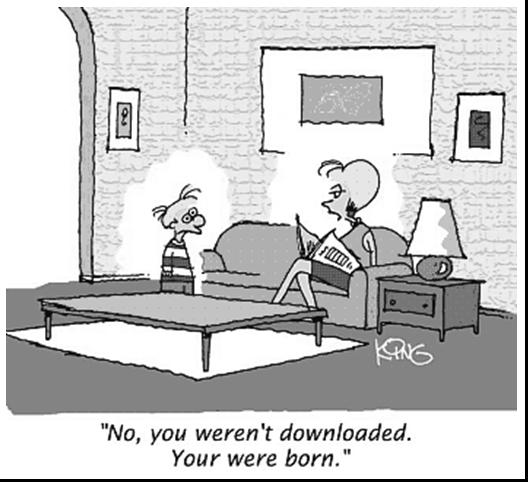
\includegraphics[width=.5\textwidth]{fig1.jpg}
%\caption{A typical figure}
%\label{fig:exampleFig1}
%\end{figure}

%\begin{figure}[ht]
%\centering
%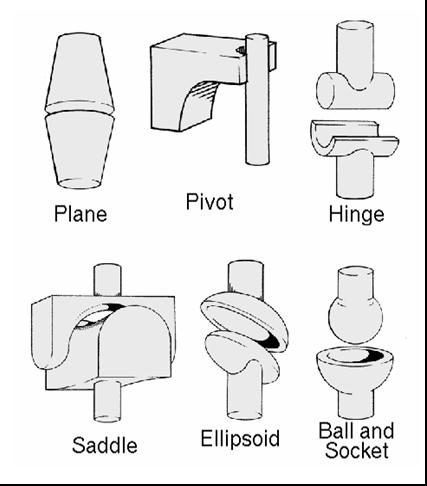
\includegraphics[width=.3\textwidth]{fig2.jpg}
%\caption{This figure is an example of a figure caption taking more than one
%  line and justified considering margins mentioned in %Section~\ref{sec:figs}.}
%\label{fig:exampleFig2}
%\end{figure}


% EXEMPLO DE TABELA

%\begin{table}[ht]
%\centering
%\caption{Variables to be considered on the evaluation of interaction  techniques}
%\label{tab:exTable1}
%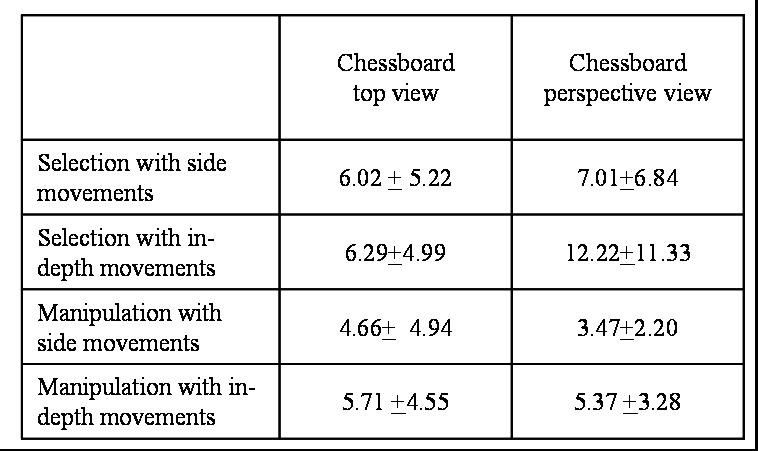
\includegraphics[width=.7\textwidth]{table.jpg}
%\end{table}



\bibliographystyle{sbc}
\bibliography{sbc-template}

\end{document}
